% ==================================================================
\section{问题二：模态局部缺失下的鲁棒情感预测}\label{sec:q2}
% ==================================================================

这一章的顺序和我们实际推进的顺序一致：先看基线在附件2上的表现，再用鲁棒性曲线和消融找它的短板，然后针对局部连续缺失做改造，最后分析缺失规律并对附件3推理。除特别注明“验证集”的结果外，本章表格中的数值均在附件2测试集上计算，且都是全量训练（3395条训练样本、200轮）后的结果。

\subsection{基线的基础性能}\label{sec:mainres}

表\ref{tab:main}给出了复现后的基线在完整模态和整模态缺失（$r=0.5$）两种条件下的结果。

\begin{table}[htbp]
\centering
\caption{基线 LDSD 的基础性能（准确率与 F1 单位为 \%）}
\label{tab:main}
\begin{tabular}{lccccccc}
\toprule
条件 & Acc-3 & F1-macro & MAE & Corr & Acc-2 & Acc-5 & Acc-7 \\
\midrule
完整模态 & 68.78 & 60.48 & 0.6628 & 0.6722 & 74.00 & 52.41 & 44.57 \\
整模态缺失 $r=0.5$ & 58.32 & 45.80 & 0.7646 & 0.4959 & 64.10 & 46.91 & 41.54 \\
\bottomrule
\end{tabular}
\end{table}

作为参照，三分类随机猜测的准确率是33.3\%，二分类约50\%。完整模态下 Acc-2 为74.00\%，文献\cite{shi2026ldsd}报告的 Acc-2 为73.48\%，两者数据集不完全相同，不能直接比高低，但处在同一量级，说明复现是可信的。MAE 为0.6628、皮尔逊相关系数为0.6722，也都明显好于随机水平。

图\ref{fig:curve}是训练过程中验证集（$r=0.5$）上的指标变化。验证集 MAE 在第10轮左右最低（约0.72），之后逐渐上升，到第110轮前后达到约0.88，最后回落到0.80附近；Acc-3 的走势与之对应，早期约53\%，后期大致在44\%～51\%之间波动。这说明在3395条训练样本上，模型训练到中后期出现了过拟合，训练轮数还有调整空间，第\ref{sec:q2err}节会再回到这一点。

\begin{figure}[htbp]
\centering
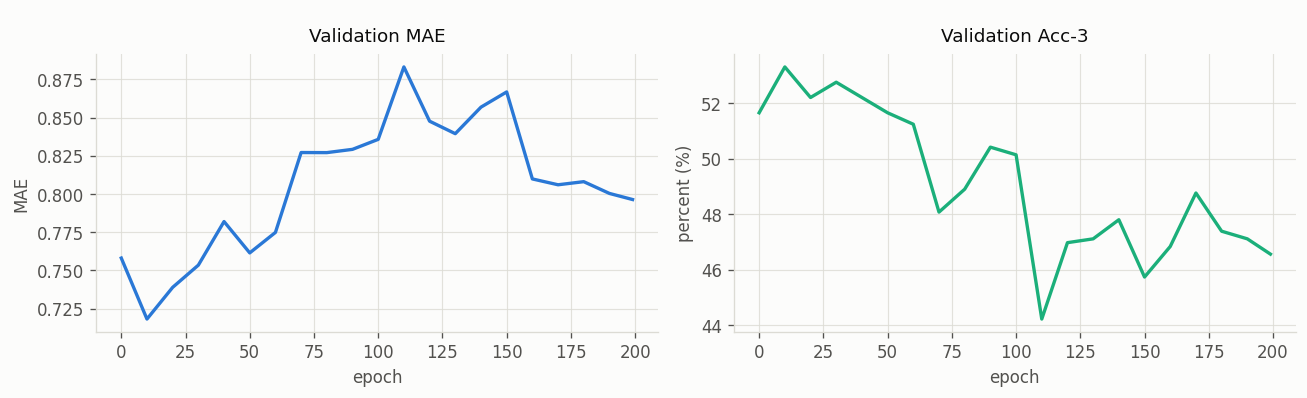
\includegraphics[width=0.92\textwidth]{figures/fig_training_curve.png}
\caption{训练过程中验证集（$r=0.5$）的 MAE（左）与 Acc-3（右）}
\label{fig:curve}
\end{figure}

\subsection{基线在整模态缺失下的鲁棒性}\label{sec:robust}

我们在整模态缺失模式下把缺失率 $r$ 从0逐步加到0.9，结果见表\ref{tab:robust}和图\ref{fig:robust}。

\begin{table}[htbp]
\centering
\caption{不同缺失率下基线的性能（整模态缺失）}
\label{tab:robust}
\begin{tabular}{lccccccc}
\toprule
$r$ & 0.0 & 0.2 & 0.4 & 0.5 & 0.6 & 0.8 & 0.9 \\
\midrule
Acc-3/\% & 68.78 & 65.47 & 62.04 & 59.56 & 56.40 & 54.33 & 50.76 \\
F1-macro/\% & 60.48 & 56.04 & 51.43 & 47.03 & 42.13 & 35.88 & 28.71 \\
MAE & 0.6628 & 0.6927 & 0.7527 & 0.7693 & 0.7750 & 0.8178 & 0.8619 \\
Corr & 0.6722 & 0.6164 & 0.5240 & 0.4883 & 0.4467 & 0.3440 & 0.2283 \\
\bottomrule
\end{tabular}
\end{table}

\begin{figure}[htbp]
\centering
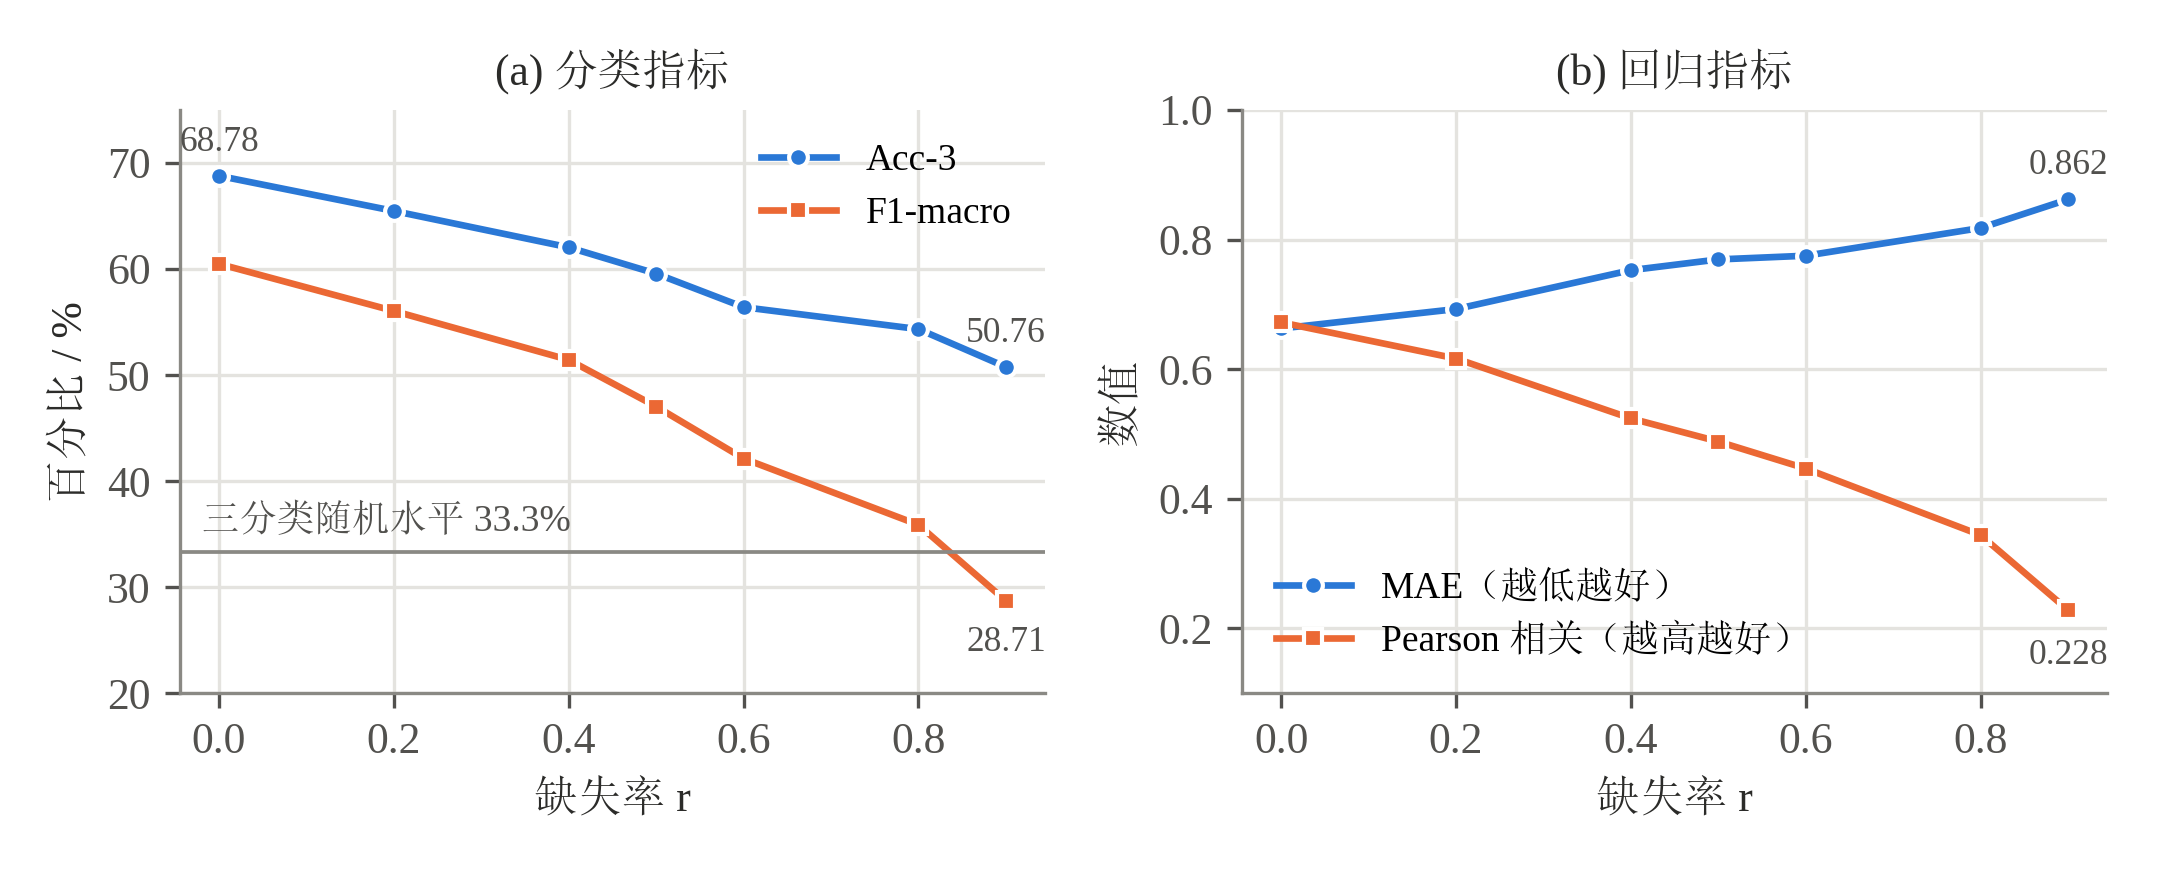
\includegraphics[width=0.95\textwidth]{figures/fig_robustness.png}
\caption{基线性能随缺失率的变化}
\label{fig:robust}
\end{figure}

整体看，性能随缺失率平滑下降，没有出现突然崩溃的拐点；即使 $r=0.9$，Acc-3 仍有50.76\%，高于随机水平。但两类指标掉得并不一样快：从 $r=0$ 到 $r=0.9$，Acc-3 下降了18.02个点，F1-macro 却下降了31.77个点，在 $r=0.9$ 时只剩28.71\%，已经低于33.3\%的随机水平。准确率还说得过去而宏平均 F1 低于随机，说明缺失严重时模型的预测集中到了少数类别上，某一类几乎不再被预测出来。这是第\ref{sec:q2err}节错误归因的第一条线索。

\subsection{三组消融：语言是不是主导，各组件有没有用}\label{sec:ablation}

LDSD 的核心主张有三条：语言不可或缺、以语言为主导模态最优、自蒸馏与重建有益。我们按这三条分别做了三组消融，每组回答一个问题，统一在 $r=0.5$ 的整模态缺失下评测。

\textbf{（1）模态消融：语言是不是不可或缺。}把某个模态的输入永久置为全缺失，并去掉它在 AHL 中的贡献，其余不变，结果见表\ref{tab:abl_mod}。

\begin{table}[htbp]
\centering
\caption{模态消融结果}
\label{tab:abl_mod}
\begin{tabular}{lccccc}
\toprule
设置 & Acc-3/\% & F1-macro/\% & MAE & Corr & F1 相对完整模型 \\
\midrule
完整模型 & 58.32 & 45.80 & 0.7646 & 0.4959 & — \\
去掉语言 & 49.79 & 22.16 & 0.8772 & 0.1620 & $-23.6$ \\
去掉语音 & 57.63 & 42.74 & 0.7643 & 0.5076 & $-3.1$ \\
去掉视觉 & 58.60 & 48.32 & 0.7578 & 0.5086 & $+2.5$ \\
\bottomrule
\end{tabular}
\end{table}

去掉语言是断崖式的：F1-macro 从45.80\%跌到22.16\%，皮尔逊相关从0.4959掉到0.1620，模型几乎失去了与人工标注的相关性。去掉语音或视觉的影响则温和得多，去掉视觉后 F1 甚至略有上升，不过幅度在正常波动范围内。

这组结果不是可有可无的对比。整个网络建立在“语言主导”的前提上，式(\ref{eq:alpha})～(\ref{eq:hyp})和式(\ref{eq:fuse})都让语言当 Query。如果去掉语言影响不大，那就说明前提是错的，后面所有围绕语言设计的模块都失去了依据。

\textbf{（2）主导模态消融：让语言当主导是不是最好的选择。}上一组只说明了语言“不能少”，没有说明“让它当主导最好”。万一让语音主导效果更好呢？所以我们把主导模态分别换成语音和视觉，即让该模态走三尺度编码、充当融合层的 Query，另外两个模态充当超模态，结果见表\ref{tab:abl_dom}。

\begin{table}[htbp]
\centering
\caption{主导模态消融结果}
\label{tab:abl_dom}
\begin{tabular}{lcccc}
\toprule
主导模态 & Acc-3/\% & F1-macro/\% & MAE & Corr \\
\midrule
语言 & \textbf{58.32} & \textbf{45.80} & \textbf{0.7646} & \textbf{0.4959} \\
语音 & 57.08 & 43.40 & 0.7736 & 0.4673 \\
视觉 & 56.67 & 45.04 & 0.7697 & 0.4744 \\
\bottomrule
\end{tabular}
\end{table}

语言主导在四项指标上全部最优。语音主导时 F1 低2.4个点、相关系数低0.029；视觉主导时 Acc-3 低1.7个点。两组合起来，才完整支撑了“语言主导”这个设计：第一组说明语言必要，第二组说明把主导权交给语言是最好的安排。

\textbf{（3）组件消融：自蒸馏和重建到底有没有用。}逐个去掉四个组件，保持其余结构不变，结果见表\ref{tab:abl_comp}。

\begin{table}[htbp]
\centering
\caption{组件消融结果}
\label{tab:abl_comp}
\begin{tabular}{lccccl}
\toprule
设置 & Acc-3/\% & F1-macro/\% & MAE & Corr & 判断 \\
\midrule
完整模型 & 58.32 & 45.80 & 0.7646 & 0.4959 & 基准 \\
去掉自蒸馏 & 56.26 & 37.48 & 0.8085 & 0.4639 & 明显退化 \\
去掉超模态融合 & 57.91 & 43.34 & 0.7772 & 0.4695 & 退化 \\
去掉重建 & 56.95 & 47.16 & 0.7538 & 0.5058 & F1、MAE 反而略好 \\
去掉 AHL & 58.32 & 46.69 & 0.7441 & 0.5098 & MAE、Corr 反而略好 \\
\bottomrule
\end{tabular}
\end{table}

结果要分两层看。正面的一层：去掉自蒸馏后 F1 下降8.3个点、MAE 上升0.044，是四个组件里影响最大的；去掉超模态融合也明显退化。这说明 EMA 教师提供的重建目标确实比单纯的自监督目标更有用，跨模态融合也是有效的。

反直觉的一层：去掉重建（MAE 0.7538）和去掉 AHL（MAE 0.7441）之后，MAE 和相关系数反而比完整模型略好。也就是说，原文“重建有益”的结论在本题数据上只得到了部分复现。我们如实报告这个结果，因为它本身有信息量。我们的理解是：在整模态缺失的设定下，一整路信号都没了，重建目标高度不确定，重建头学到的更像是一种“均值式”的补偿，反而冲淡了判别信号；去掉 AHL 后 MAE 更好，则说明样本级缺失时，AHL 学到的注意力权重可能引入了噪声。

这组结果直接推动了我们后面的两个决定。一是把训练时的缺失模拟改成连续段形态：整模态缺失下这两个模块表现不稳，恰恰说明“缺失的形态”很关键。二是让重建结果真正进入推理路径：如果重建只是算一个损失就被丢掉，它学不到有用的东西也就不奇怪了。第\ref{sec:m4}节的 M4 就是这样来的。

\subsection{面向局部连续缺失的改进}\label{sec:improve}

\subsubsection{缺失的形式化}\label{sec:missdef}

用掩码 $M_m\in\{0,1\}^T$ 描述模态 $m$ 的缺失，$M_m[t]=1$ 表示第 $t$ 帧不可用。注入缺失后，语音和视觉按 $U_m^1=U_m^0\odot(1-M_m)$ 置零，语言的缺失帧替换为可学习的 \texttt{[UNK]} 向量。按掩码的生成方式，可以区分三种缺失模式：
\begin{equation}\label{eq:modes}
M_m[t]=\begin{cases}
b_m,\quad b_m\sim\mathrm{Bernoulli}(r), & \text{整模态丢弃（sample）},\\[2pt]
b_{m,t},\quad b_{m,t}\overset{\text{i.i.d.}}{\sim}\mathrm{Bernoulli}(r), & \text{逐帧独立丢弃（token）},\\[2pt]
\mathbb{1}\big[t\in\mathcal{M}_m\big],\quad \mathcal{M}_m\ \text{为若干连续区间之并}, & \text{连续段缺失（segment）}.
\end{cases}
\end{equation}
前两种是基线代码实际使用的模式，第三种才是附件3中的形态。三种模式下 $r$ 的含义不同：整模态模式中是一个模态被整条丢弃的概率，后两种模式中是缺失帧所占的比例。

\subsubsection{M1：连续段缺失增强}

文献\cite{shi2026ldsd}第3.2节的文字描述是“随机遮蔽片段”（randomly masking segments），但我们阅读其公开代码后发现，实际实现是逐帧独立的伯努利采样，与“连续段”并不是一回事。这个差别在散点缺失下看不出来，换成连续段就会暴露（见第\ref{sec:screen}节，相差9.4个点）。因此我们显式构造连续段：
\begin{equation}\label{eq:m1}
\begin{gathered}
(\rho_1,\dots,\rho_k)\sim\mathrm{Dirichlet}(0.6\cdot\mathbf{1}_k),\qquad
\ell_j=\max\big(1,\ \lfloor\rho_j\, rT\rfloor\big),\\
\mathcal{M}_m=\bigcup_{j=1}^{k}\big[a_j,\ a_j+\ell_j\big),
\end{gathered}
\end{equation}
其中段数 $k\sim\mathcal{U}\{1,2,3\}$，$\ell_j$ 为第 $j$ 段的长度，各段在互不相交的区块内选取起点 $a_j$。

用 Dirichlet 分布分配段长，是为了让段长有足够的区分度：短段可以借邻域插值补回来，长段不行；如果生成的段长都差不多，评测时按段长分桶就看不出差异。这一点我们在调试阶段实际吃过亏：第一版的段长分布没有调好，93\%的样本都落进了“长段”桶，分桶结果什么也说明不了。最终浓度参数取0.6：浓度小于1时，各段分到的长度差异更大，更容易同时产生很短和很长的缺失段。

\subsubsection{M4：超模态补洞}\label{sec:m4}

文献\cite{shi2026ldsd}第3.1节的概述中说重建出的模态特征被用于语言主导的预测，但从其式(6)～(8)看，重建结果只参与了 $\mathcal{L}_{rec}$ 的计算，并没有进入推理路径。对连续段缺失来说，这个区别是决定性的：模型必须在洞里显式地填入推断出的表征，而不能指望下游模块自己学会忽略这个洞。因此我们补上这条通路：
\begin{equation}\label{eq:inpaint}
H_{Hyp}\leftarrow H_{Hyp}\odot(1-m)+E_{rec}\big(H_{Hyp}\big)\odot m,\qquad m=\max\big(M_a,M_v\big),
\end{equation}
即在语音或视觉任一模态缺失的帧上，用重建器的输出替换超模态表示，其余帧保持不变。这样重建器一方面仍受式(\ref{eq:lrec})的自蒸馏监督，另一方面它的输出直接影响预测，梯度会把“补得像不像”和“预测得准不准”绑在一起。

\subsubsection{其余三个候选模块}

除 M1 和 M4 外，我们还准备了另外三个候选，思路都是“让模型知道哪里缺了”：
\begin{itemize}
\item \textbf{M2 有效性 token}：为“缺失”和“填充”两种状态各设一个可学习向量，叠加到对应帧上，让模型能区分“本来没有”和“丢了”。
\item \textbf{M3 掩码加权损失}：把式(\ref{eq:lrec})的重建损失限制在缺失位置上计算，想让重建头把力气用在洞上。
\item \textbf{M5 掩码注意力}：在 AHL 的式(\ref{eq:alpha})(\ref{eq:beta})中屏蔽缺失帧对应的 Key/Value。
\end{itemize}
这五个模块哪个有用，我们事先并没有把握，所以决定全部实现，用数据决定去留。

\subsection{候选模块的逐级筛选}\label{sec:screen}

\textbf{筛选规则。}把模块逐个叠加上去，每加一个就与当前最好的配置比较一次边际增益；没有增益或者有损就淘汰，下一个模块仍然叠加在最后一个有效配置上。

\textbf{评测掩码。}所有配置统一用一套固定的分层连续段掩码评测：短段（最长缺失段 $\le5$ 帧）占40\%、中段（6～15帧）占35\%、长段（$>15$帧）占25\%。所有配置共用同一套掩码，并按样本中最长缺失段的长度分桶统计，这样不同配置之间才可比。评价时同时看三个量：段缺失下的 F1-macro、长段缺失下的 MAE，以及完整模态下的 F1-macro（用来确认改进没有伤害完整输入时的表现）。

先看 M1 单独的作用（表\ref{tab:m1}）。这组实验只改训练时的缺失模拟方式，把逐帧散点换成连续段，其余完全不变。

\begin{table}[htbp]
\centering
\caption{连续段缺失增强（M1）的作用}
\label{tab:m1}
\begin{tabular}{lccc}
\toprule
配置 & 段缺失 F1-macro/\% & 长段 MAE & 完整模态 F1-macro/\% \\
\midrule
基线（逐帧散点训练） & 47.63 & 0.7168 & 56.65 \\
+M1（连续段训练） & \textbf{57.03} & \textbf{0.6666} & \textbf{57.65} \\
\bottomrule
\end{tabular}
\end{table}

仅仅改变训练时的缺失模拟方式，段缺失 F1 就提升了9.4个点，长段 MAE 下降0.050，完整模态下的 F1 也没有退化（56.65\%$\to$57.65\%）。这证实了我们一开始的判断：连续段缺失和散点缺失是两种不同的失效模式，模型必须专门见过才会应对。而且 M1 不改网络结构，只改训练数据的构造方式，是性价比最高的一项。

接着在 M1 之上逐个叠加其余四个模块，结果见表\ref{tab:screen}和图\ref{fig:screen}。

\begin{table}[htbp]
\centering
\caption{候选模块逐级筛选结果}
\label{tab:screen}
\begin{tabular}{lcccl}
\toprule
配置 & 段缺失 F1/\% & 长段 MAE & 完整模态 F1/\% & 结论 \\
\midrule
M1（参照） & 57.03 & 0.6666 & 57.65 & 基准 \\
M1+M2 & 57.25 & 0.6702 & 57.92 & 增益在噪声内，淘汰 \\
M1+M3 & 56.37 & 0.6865 & 56.92 & 有害，淘汰 \\
M1+M4 & \textbf{60.21} & \textbf{0.6572} & \textbf{60.86} & 保留 \\
M1+M4+M5 & 58.02 & 0.6708 & 56.81 & 有害，淘汰 \\
\bottomrule
\end{tabular}
\end{table}

\begin{figure}[htbp]
\centering
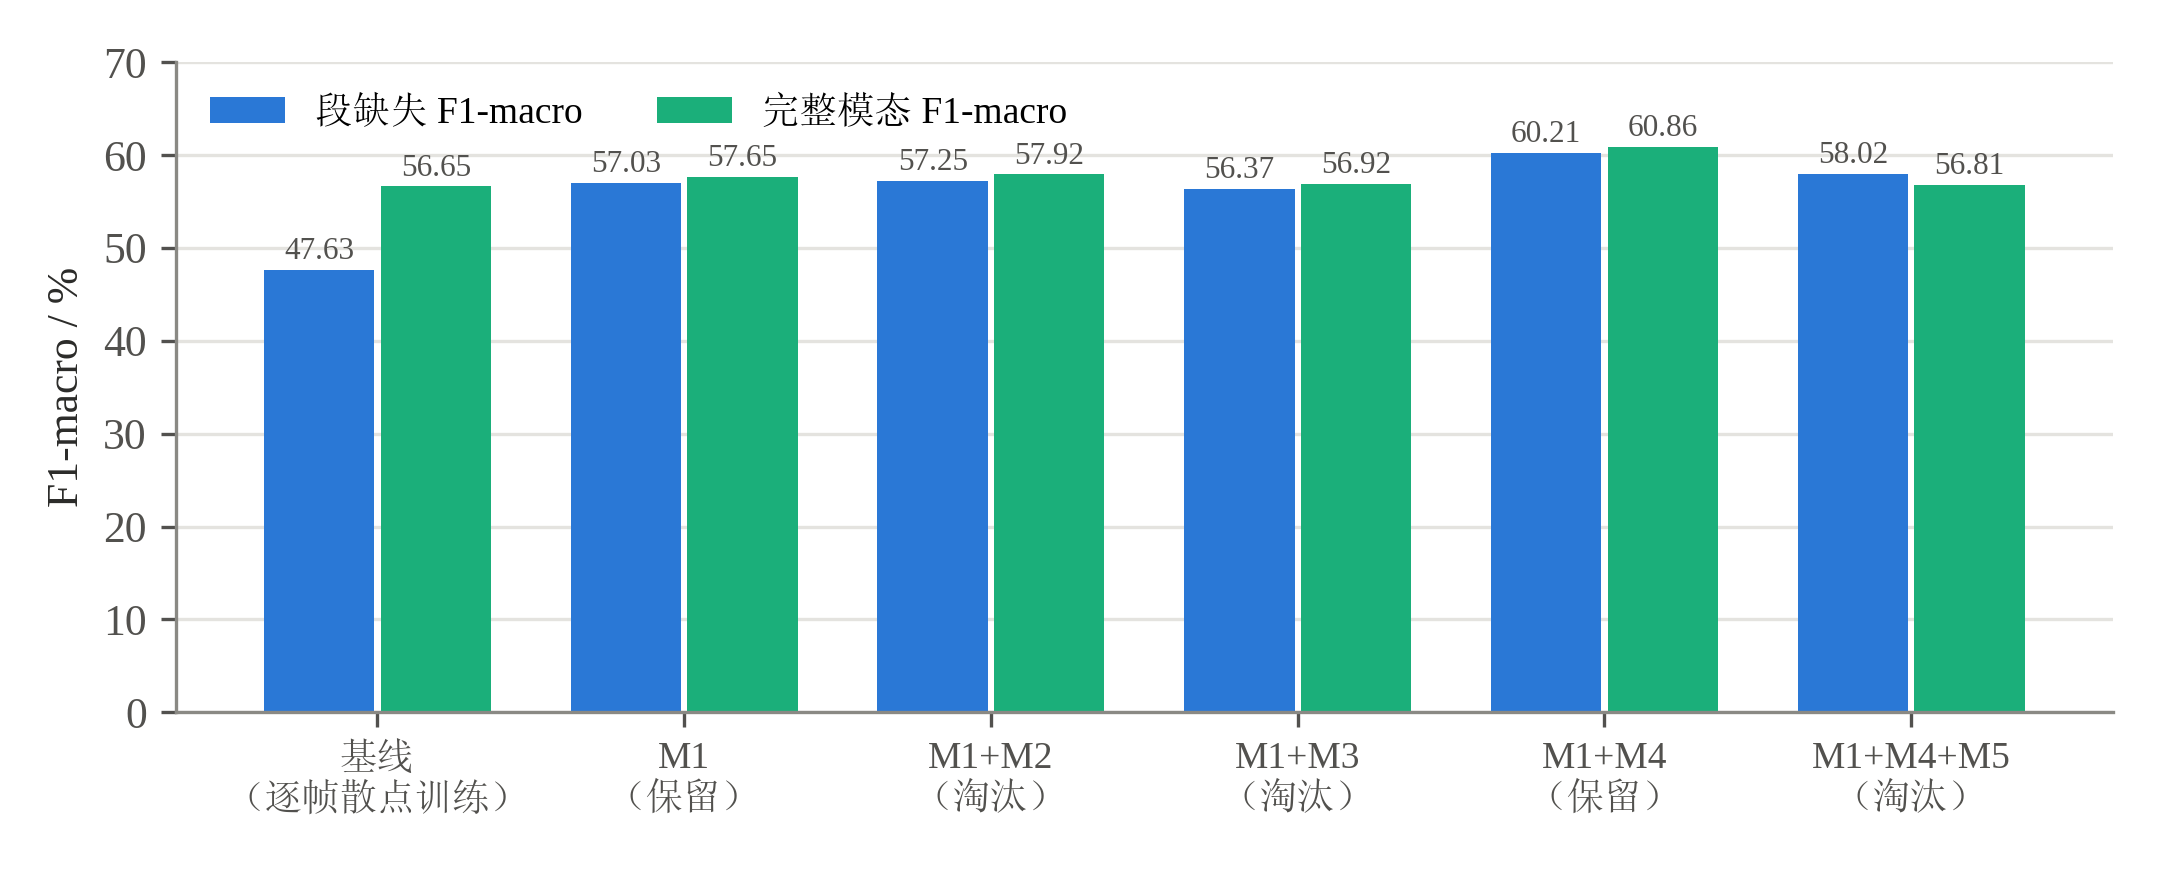
\includegraphics[width=0.95\textwidth]{figures/fig_module_screen.png}
\caption{候选模块筛选过程中段缺失与完整模态下的 F1-macro}
\label{fig:screen}
\end{figure}

只有 M4 带来了实质增益：段缺失 F1 提升3.2个点，完整模态 F1 同步提升3.2个点，长段 MAE 下降0.009。其余三个都没有通过：

M2 的 F1 只比参照高0.22个点，长段 MAE 反而从0.6666变差到0.6702，这点增益在噪声范围内，不足以成为保留的理由。

M3 明确有害。事后分析原因：把重建损失限制到缺失位置后，监督信号变得很稀疏，重建头在观测帧上失去了约束，开始“漂移”。本想让损失更聚焦，结果削弱了整体约束。

M5 同样有害。屏蔽掉大量 Key/Value 之后，注意力可用的上下文反而变少了，完整模态 F1 和长段 MAE 都比 M1+M4 差。

这里有一个流程上的教训值得单独记下。M3 判定失败时，我们原先已经把 M4、M5 叠在“M1+M3”这个坏配置上跑了一轮，那一轮结果完全不可用，只好回到最后一个有效配置 M1 上重跑，才判定出 M4 有效。如果省掉这次重跑，M4 的增益会被 M3 的损害掩盖掉，很可能被误判为无效。

回头看这组筛选，M2 和 M5 都是在给模型提供“哪里缺了”的额外信息，但都没用；真正起作用的 M4 不只是告诉模型洞在哪，而是直接把洞填上。最终保留 M1 与 M4，记为 LDSD-Seg。

\subsection{训练方案与关键参数}

表\ref{tab:params}列出了 LDSD-Seg 的主要配置。结构参数与文献\cite{shi2026ldsd}保持一致，缺失相关的参数由第\ref{sec:screen}节的筛选确定。

\begin{table}[htbp]
\centering
\caption{LDSD-Seg 的训练方案与关键参数}
\label{tab:params}
\begin{tabular}{>{\raggedright\arraybackslash}p{3.6cm}>{\raggedright\arraybackslash}p{9.2cm}}
\toprule
项目 & 设置 \\
\midrule
训练数据 & 附件2 aligned\_50.pkl 训练集3395条；验证集用于选择结构与阈值 \\
序列与维度 & $T=50$，$d=128$，8头注意力，$d_k=16$ \\
语言多尺度编码 & 在 $H_l^1$ 上叠加两层8头 Transformer \\
重建器 $E_{rec}$ & 两层8头 Transformer + 线性输出层 \\
自蒸馏 & 教师为学生参数的 EMA，$\eta=0.99$ \\
损失权重 & $\lambda=0.5$，$\gamma=1.0$，$\mathcal{L}_{sp}=\mathcal{L}_{reg}+\mathcal{L}_{cls}$ \\
缺失增强（M1） & 段数 $k\sim\mathcal{U}\{1,2,3\}$，段长按 Dirichlet$(0.6)$ 分配 \\
补洞（M4） & $m=\max(M_a,M_v)$，见式(\ref{eq:inpaint}) \\
训练轮数 & 200轮 \\
优化器、学习率、批大小 & \todo{从配置文件抄录} \\
运行环境与耗时 & Kaggle GPU；全部实验总耗时 7772.6 s（约2.16 h） \\
\bottomrule
\end{tabular}
\end{table}

\subsection{LDSD-Seg 的全量确认}\label{sec:segconfirm}

筛选阶段的结论要在最终配置上再确认一次。我们把基线（整模态缺失增强，无补洞）与 LDSD-Seg 放在同一套固定分层连续段掩码下评测。用同一套掩码是关键，否则两者面对的缺失样本不同，数字没法比。结果见表\ref{tab:seg}和图\ref{fig:seg}。

\begin{table}[htbp]
\centering
\caption{局部连续缺失下基线与 LDSD-Seg 的对比}
\label{tab:seg}
\begin{tabular}{lcccccc}
\toprule
\multirow{2}{*}{配置} & \multicolumn{3}{c}{段缺失（整体）} & \multicolumn{3}{c}{按最长缺失段分桶的 MAE} \\
\cmidrule(lr){2-4}\cmidrule(lr){5-7}
 & MAE & F1/\% & Acc-3/\% & 短段 & 中段 & 长段 \\
\midrule
基线 LDSD & 0.7112 & 47.26 & 63.82 & 0.6780 & 0.7034 & 0.7205 \\
LDSD-Seg & \textbf{0.6639} & \textbf{61.70} & \textbf{67.81} & \textbf{0.6175} & \textbf{0.6849} & \textbf{0.6548} \\
变化量 & $-0.047$ & $+14.4$ & $+4.0$ & $-0.061$ & $-0.019$ & $-0.066$ \\
\bottomrule
\end{tabular}
\end{table}

\begin{figure}[htbp]
\centering
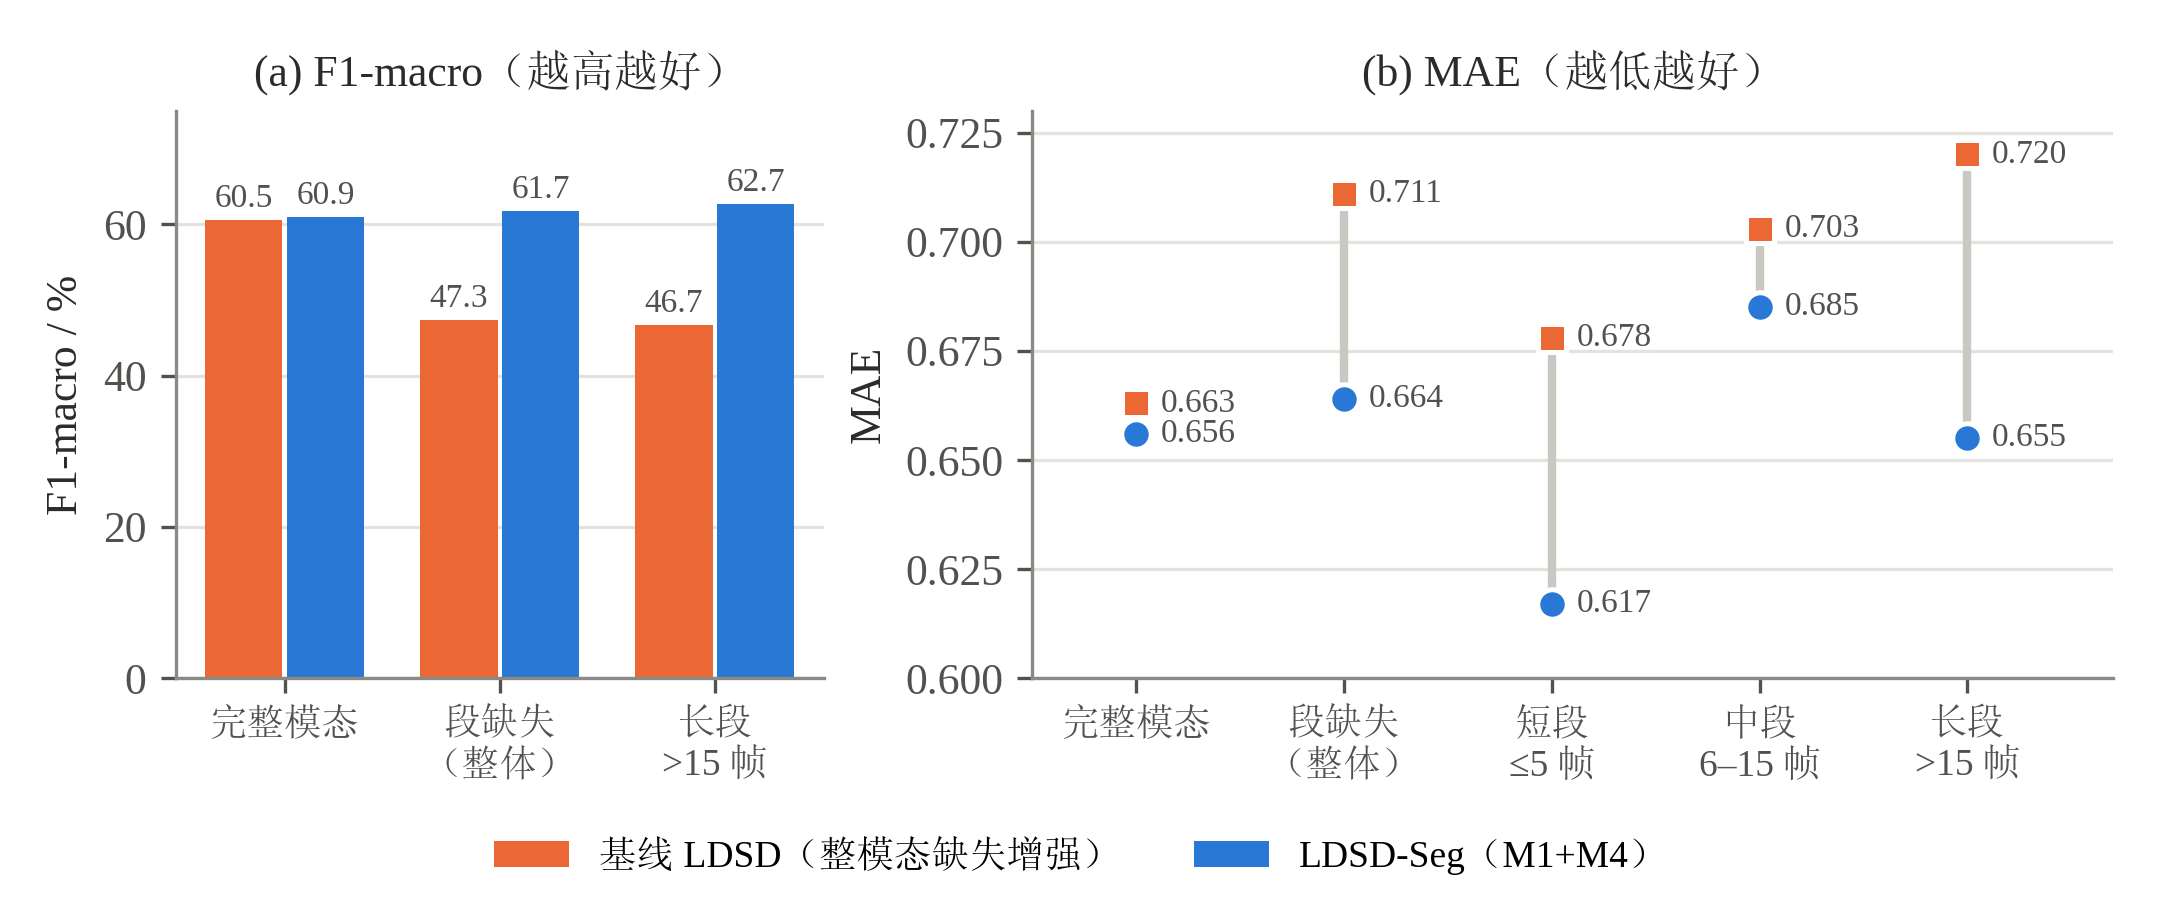
\includegraphics[width=0.95\textwidth]{figures/fig_segment_compare.png}
\caption{同一套分层连续段掩码下，基线与 LDSD-Seg 的 F1-macro（a）和 MAE（b）}
\label{fig:seg}
\end{figure}

段缺失 F1 从47.26\%提升到61.70\%，MAE 从0.7112降到0.6639。分桶看，长段 MAE 的降幅（0.066）大于整体（0.047），说明改进确实作用在最难的情形上，而不是靠容易的样本刷分。不过中段的改善最小，只有0.019，这一点我们目前还没有找到令人满意的解释，只能如实列出。

比起绝对性能，“缺失让性能掉了多少”更能说明鲁棒性。表\ref{tab:gap}是验证集上完整模态与段缺失之间的落差。

\begin{table}[htbp]
\centering
\caption{验证集上完整模态与段缺失之间的 F1-macro 落差}
\label{tab:gap}
\begin{tabular}{lccc}
\toprule
模型 & 完整模态 F1/\% & 段缺失 F1/\% & 落差 \\
\midrule
基线 LDSD & 55.56 & 39.93 & $-15.6$ \\
LDSD-Seg & 59.36 & \textbf{59.47} & $+0.1$ \\
\bottomrule
\end{tabular}
\end{table}

基线一遇到连续段缺失就掉15.6个点，LDSD-Seg 在同样条件下几乎不掉（$+0.1$，在波动范围内）。我们最初的动机只是“题目要求处理局部缺失”，但真正让我们决定保留这两个模块的依据是这个落差：它比绝对性能更直接地反映了鲁棒性有没有真的改善。

还要说明一点：同一个 M1+M4 配置，在筛选实验中段缺失 F1 为60.21\%，在这里为61.70\%，两次运行相差约1.5个点。这提示单次运行的结果存在一定波动，表中小于1个点左右的差异不宜过度解读。

\subsection{缺失类型、位置与时长的影响规律}\label{sec:factor}

\subsubsection{实验设计}

题目要求分析缺失模态类型、缺失位置、缺失时长对性能的影响。我们做了三因子扫描：
\begin{itemize}
\item 模态类型：$\{l,a,v\}$ 的6个非空真子集，即 $l$、$a$、$v$、$l{+}a$、$l{+}v$、$a{+}v$；
\item 位置：缺失段位于内容的前部（head）、中部（mid）、尾部（tail）；
\item 时长：$\rho\in\{0.10,0.25,0.50,0.75,0.90,1.00\}$，$\rho$ 为缺失段占该模态自身内容跨度的比例。
\end{itemize}
共 $6\times3\times6=108$ 个单元。模型固定为训练好的 LDSD-Seg，只训练一次，所有因子组合都只在评测时构造掩码、重新跑前向，因此108个单元不需要训练108次，扫描本身只占全部耗时的1～2分钟。指标为相对完整模态的 MAE 增量 $\Delta\mathrm{MAE}$。

\subsubsection{设计中修正的两处错误}

这两处错误都是靠事先设置的校验项抓出来的，这里单独交代一下。

\textbf{位置不能用绝对帧号。}我们最初统一用语音的有效长度 $L_a$ 来划分所有模态的前、中、尾部。结果对文本来说只遮蔽了前21帧左右，剩下的帧照样能读出情感，实测文本缺失的 $\Delta\mathrm{MAE}$ 竟然是负的，差点得出“语言缺失无害”这个完全错误的结论。正确做法是每个模态按自身的内容跨度取相对坐标。

\textbf{$\rho$ 必须铺到1.0。}各模态的冗余度不同，同一个 $\rho$ 下的绝对损失量不可比。第一版的时长只取到0.75，什么规律都看不出来；把范围扩展到0.90和1.00后，规律才显现出来。

\subsubsection{校验：语言全缺时必须最差}

在进入正式分析之前，先在 $\rho=1.0$（整模态全部遮蔽）上做一次校验，记为 H1：既然第\ref{sec:ablation}节已经证明语言不可或缺，那么语言全缺时的损失理应最大。结果见表\ref{tab:h1}。

\begin{table}[htbp]
\centering
\caption{校验 H1：$\rho=1.0$ 时各模态组合缺失的 $\Delta\mathrm{MAE}$}
\label{tab:h1}
\begin{tabular}{lcccccc}
\toprule
缺失模态 & $l$ & $l{+}a$ & $l{+}v$ & $a$ & $v$ & $a{+}v$ \\
\midrule
$\Delta\mathrm{MAE}$ & $+0.789$ & $+0.764$ & $+0.752$ & $+0.003$ & $+0.004$ & $+0.006$ \\
\bottomrule
\end{tabular}
\end{table}

语言缺失的 $\Delta\mathrm{MAE}$ 约为语音、视觉的200倍（0.789对0.004），校验成立。这组数不算新发现，它和模态消融的结论一致，本就在预料之中。它的作用是检查扫描代码有没有写对：如果这里语言不是最差的，就说明坐标定义或掩码构造有 bug。事实证明这个担心不多余，上一小节的两处错误，都是因为这项校验不成立才被发现的。因子扫描是新写的代码，一旦实现有误，错误的结论就会被当成“发现”写进报告，所以我们先设了一个已知答案的检查项。

\subsubsection{时长的影响}

表\ref{tab:dur}给出了时长的主效应及其在各模态上的分解，图\ref{fig:factor}是对应的曲线。

\begin{table}[htbp]
\centering
\caption{不同缺失时长下的 $\Delta\mathrm{MAE}$}
\label{tab:dur}
\begin{tabular}{lcccccc}
\toprule
$\rho$ & 0.10 & 0.25 & 0.50 & 0.75 & 0.90 & 1.00 \\
\midrule
全部模态平均 & $+0.003$ & $+0.005$ & $+0.008$ & $+0.016$ & $+0.033$ & $+0.386$ \\
语言 $l$ & $+0.005$ & $+0.008$ & $+0.012$ & $+0.027$ & $+0.060$ & $+0.789$ \\
语音 $a$ & $+0.001$ & $+0.001$ & $+0.002$ & $+0.003$ & $+0.003$ & $+0.003$ \\
视觉 $v$ & $+0.000$ & $+0.001$ & $+0.000$ & $+0.000$ & $+0.000$ & $+0.004$ \\
\bottomrule
\end{tabular}
\end{table}

\begin{figure}[htbp]
\centering
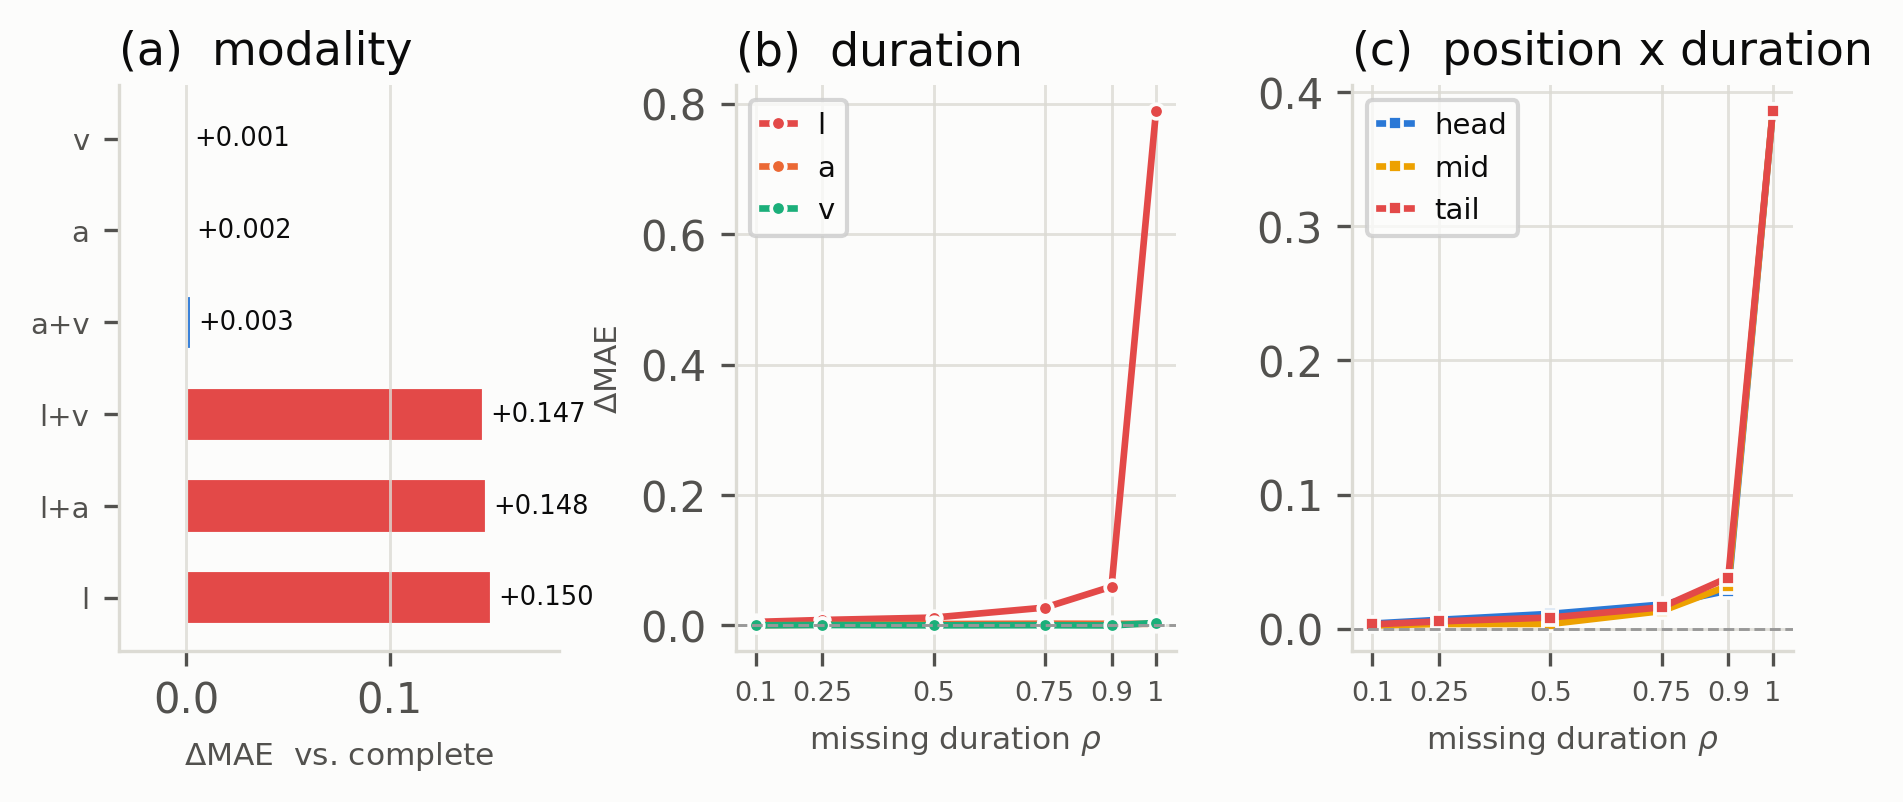
\includegraphics[width=\textwidth]{figures/fig_factor_scan.png}
\caption{三因子扫描结果：(a) 各模态组合的平均 $\Delta\mathrm{MAE}$；(b) 各模态 $\Delta\mathrm{MAE}$ 随时长的变化；(c) 不同位置下 $\Delta\mathrm{MAE}$ 随时长的变化}
\label{fig:factor}
\end{figure}

拆到各模态看，规律完全不同。语言呈现“全有或全无”的形态：缺失90\%以内几乎无感（$\rho=0.9$ 时 $\Delta\mathrm{MAE}$ 仅0.060），一旦接近全缺就断崖式崩溃（$\rho=1.0$ 时为0.789，是前者的13倍）。语音、视觉则全程平缓，始终低于0.006。

我们对语言这种形态的理解是：文本特征是 BERT 的上下文表示，每一帧都编码了整句的信息，即使在补齐位置上也不为零（表\ref{tab:zero}中文本零帧比例为0）。所以只要还剩一部分文本帧，模型就能从中读出整句的情感；也正因为冗余度高，剩余信息一旦不足，就再没有冗余可退，崩溃是断崖式的。语音、视觉的有效帧少（中位21帧）、冗余度低，信息随缺失线性流失，贡献也小，所以曲线平缓。

\subsubsection{位置的影响}

表\ref{tab:pos}按缺失位置分组（每组36个单元）给出了平均 MAE。

\begin{table}[htbp]
\centering
\caption{不同缺失位置下的平均 MAE}
\label{tab:pos}
\begin{tabular}{lccc}
\toprule
位置 & 前部 head & 中部 mid & 尾部 tail \\
\midrule
MAE & 0.7319 & 0.7296 & 0.7324 \\
\bottomrule
\end{tabular}
\end{table}

三者相差不到0.003，远小于时长效应（0.386）。我们原本猜测“句子中部的缺失最要命”，这个假设被数据否定了。这可能与数据的词级对齐有关：序列不是按时间等距采样的，每一帧就是一个词，而情感线索在句中的分布并没有明显的位置偏好；再加上文本帧都是上下文表示，缺了哪一段，其余帧里多少都还留着这段的信息。

\subsubsection{规律小结}

三因子扫描的结论可以归纳为三句话：时长是主因，而不是位置，也不单是“哪个模态”；语言缺失90\%以内几乎无感，接近全缺时 $\Delta\mathrm{MAE}$ 陡增13倍；位置的影响可以忽略。落到应用上，在90\%以内的缺失预算下，应优先保证语言不被整段丢掉，而不必纠结缺失发生在句子的哪个位置。换句话说，“丢了多少”比“丢在哪里”重要得多。

\subsection{附件3的推理结果}\label{sec:att3}

附件3的推理流程与训练时的预处理完全一致：先用 bert-base-uncased 把 text\_bert 重建为文本特征，在标准化之前计算各模态有效长度，再用训练集统计量对语音、视觉做 z-score，最后送入 LDSD-Seg。每条样本输出极性、极性置信度（三分类概率的最大值）、强度和主导模态。30条样本的汇总见表\ref{tab:att3}，逐条结果见附录\ref{app:att3}，分布见图\ref{fig:att3}。

\begin{table}[htbp]
\centering
\caption{附件3推理结果汇总}
\label{tab:att3}
\begin{tabularx}{\textwidth}{lX}
\toprule
项目 & 结果 \\
\midrule
极性分布 & 正向14条，负向11条，中性5条 \\
极性置信度均值 & 0.703 \\
预测强度均值 & $-0.077$ \\
主导模态 & 文本28条；例外为附件3\_14（视觉主导）和附件3\_17（语音主导） \\
\bottomrule
\end{tabularx}
\end{table}

\begin{figure}[htbp]
\centering
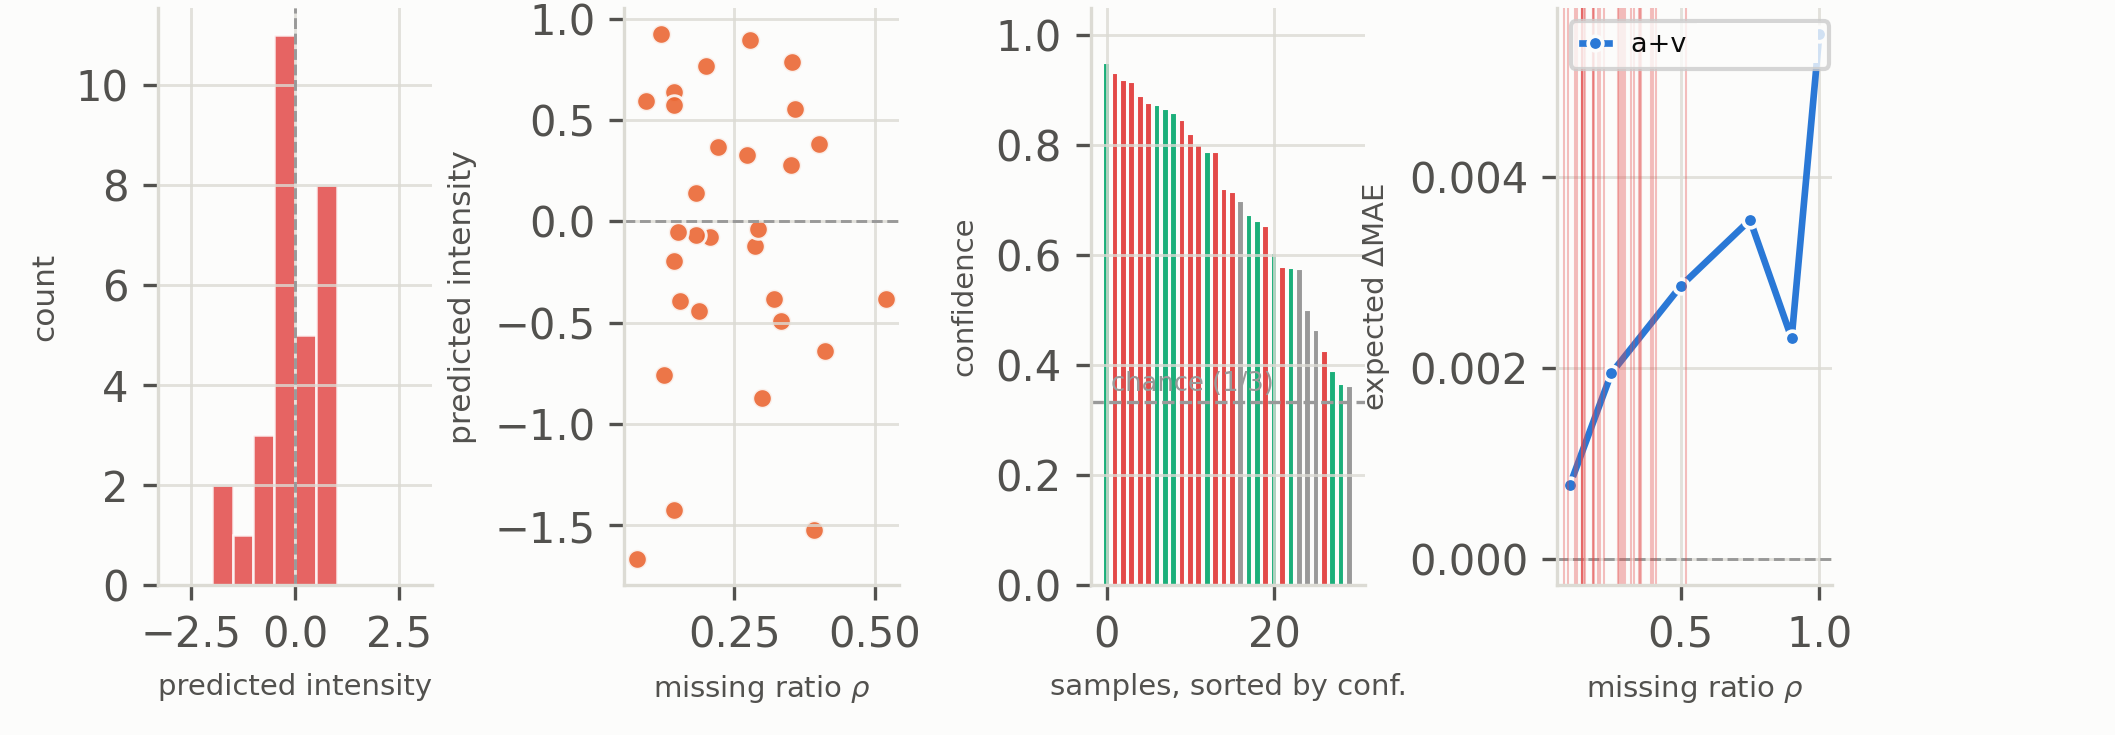
\includegraphics[width=\textwidth]{figures/fig_att3.png}
\caption{附件3推理结果：(a) 预测强度分布；(b) 缺失比例与预测强度；(c) 按置信度排序的极性置信度（红、绿、灰分别为正向、负向、中性）；(d) 各样本缺失比例（竖线）与因子扫描中 $a{+}v$ 缺失的预期 $\Delta\mathrm{MAE}$ 曲线}
\label{fig:att3}
\end{figure}

有几点观察。第一，附件3的缺失全部落在语音和视觉上，缺失比例 $\rho$ 都不超过0.55。对照因子扫描中 $a{+}v$ 缺失的曲线（图\ref{fig:att3}(d)），这个范围内预期的 $\Delta\mathrm{MAE}$ 不超过0.003，远没有到语言的断崖区，所以附件3的缺失对预测的影响应当很小；图\ref{fig:att3}(b)中预测强度与缺失比例之间也看不出明显的趋势。第二，5条中性预测里有4条排在置信度最低的7条之内，中性样本最不“确定”，这与第\ref{sec:robust}节 F1 掉得比准确率快的现象是吻合的。第三，附件3\_14 和附件3\_17 两条的主导模态不是文本，这在30条里比较特殊，建议人工回看。

需要强调的是，附件3没有标签，上面这些只能说明模型输出是否“合理”，不能说明它是否“正确”。附件3预测结果的可信度，主要取决于模型在附件2上的表现。

\subsection{验证集上的错误归因}\label{sec:q2err}

综合前面几节的结果，模型的错误主要来自以下几个方面。

\textbf{（1）类别之间不均衡，缺失越重越明显。}各种条件下 F1-macro 都明显低于 Acc-3；缺失率升高时 F1 掉得更快，$r=0.9$ 时低于随机水平而 Acc-3 仍有50.76\%，说明预测向少数类别集中。附件3中中性预测的置信度普遍偏低，也指向同一个问题：中性与弱正、弱负之间的边界是模型最拿不准的地方。

\textbf{（2）语言接近全缺时误差陡增。}三因子扫描显示，误差几乎全部集中在语言缺失比例接近1的情形，$\rho$ 从0.9到1.0，$\Delta\mathrm{MAE}$ 由0.060跳到0.789。对于只丢语音、视觉的样本，模型几乎不受影响。

\textbf{（3）训练后期过拟合。}图\ref{fig:curve}中验证集 MAE 在第10轮左右最低，之后整体上升，Acc-3 同步下降。3395条训练样本对这样规模的网络来说偏少，固定训练200轮并不是最优的选择。

\textbf{（4）整模态缺失下重建模块的补偿偏“平均”。}组件消融中去掉重建、去掉 AHL 反而略好，说明在一整路信号都缺失时，重建出的内容更接近均值，稀释了判别信息。这也是我们改用连续段训练、并让重建结果进入推理路径的原因。

\subsection{小结}

问题二的核心发现是：题目要求的局部连续缺失在训练数据中基本不存在，照搬文献的缺失设定训练出的鲁棒性并不可靠。围绕这一点，我们从5个候选中筛出了连续段缺失增强（M1）与超模态补洞（M4）两个模块，在同一套分层连续段掩码下把段缺失 F1 从47.26\%提升到61.70\%，验证集上完整模态与段缺失之间的落差从15.6个点缩小到0.1个点。三因子扫描进一步说明，缺失时长是影响性能的主因，语言缺失呈“全有或全无”的形态，位置的影响可以忽略。
